\section{Dinics}

\subsection{Sequential Algorithm}
    \subsubsection{Introduction}
    Dinic's algorithm is a flow algorithm that was created by Dr. Yefim Dinitz, and is notable for being strongly polynomial with an $\mathcal{O}(V^2E)$ run-time. Dinic's algorithm innovates on other flow algorithms with its use of level graphs and blocking flows. Dinic's algorithm uses BFS and DFS in order to achieve this superior run-time; bread-first search for building a level graph, and depth-first search with blocking flows in order to find the maximum flow efficiently.

    \subsubsection{Algorithm Overview}
       In what follows, we are going to walk the through the algorithm, step by step, with examples from our own implementation. \emph{To provide a brief overview of the original Dinic's algorithm, the pseudo-code has been provided below.}
       
    \begin{description}
        \item[] Input: A network G = ((V, E), c, s, t).
        \item[] Output: An s-t flow f of maximum value.  
    \end{description}    
    \begin{enumerate}
        \item Set $f(e) = 0$ for each $e \in E.$
        \item Construct $G_L$ from $G_f$ of G. If $dist(t)=\infty$, stop and output f.
        \item The text in the entries may be of any length.
    \end{enumerate}
    
    % \subsection{}
    The algorithm begins with the assumption that we want to make positive progress from the source node towards the sink node. We achieve this goal by using a level graph (Figure 11),
    
    \begin{figure}[H]
        \centering
        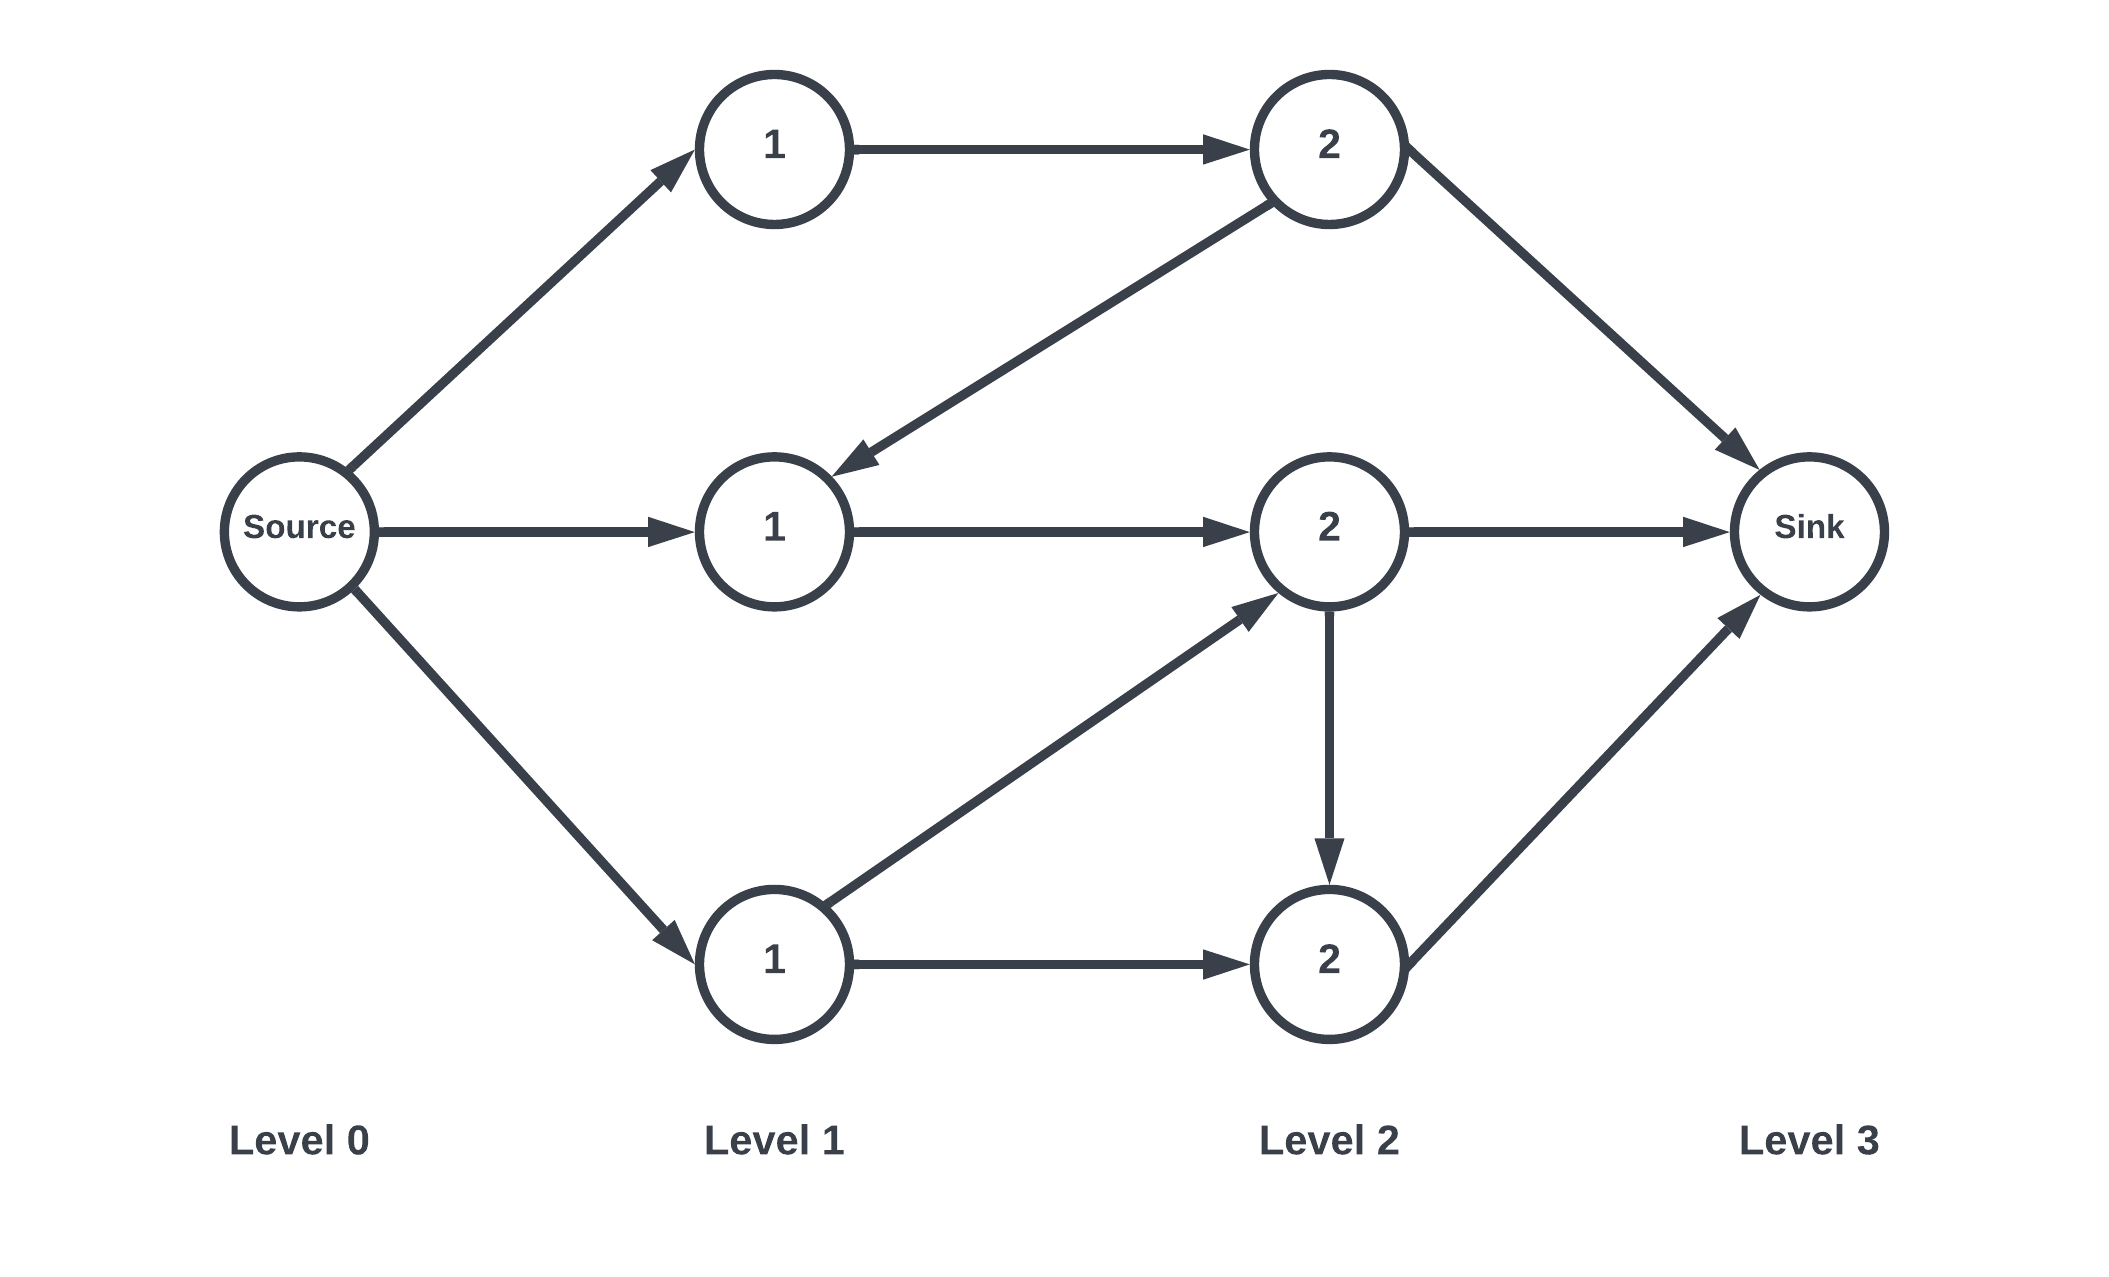
\includegraphics[scale=0.13, center]{figures/NetworkFlow_Dinics-4.png}
        \caption{Network Flow Graph}
    \end{figure}
    
    which keeps track of whether the edges are making progress towards the sink or not. This level graph is built using BFS, since with BFS we can easily calculate the minimum distance, or level, from the source node to other nodes. BFS achieves this by looking at the directed edges that point toward neighboring nodes from the current node, and if a level has not been set for those nodes, a level will be assigned. The neighboring nodes will get added to a queue for the next iteration of the BFS, where the same steps will take place, except this time, we will be setting the next set of neighboring nodes to level + 1. \cite{williamfiset} \emph{See pseudo-code below for a more detailed overview of how the Dinic's BFS would create a level graph:}
    
    \begin{algorithm}
        \caption{BFS Pseudo Code}
        \label{alg:BFS}
        \begin{algorithmic}[1]
            \State Node:
                \State $level \gets$ Integer
                \State $edges \gets$ Array of nodes\
                \State $capacityRemaining \gets$ Integer
                
            \Function{BFS}{} 
                \State $queue \gets$ empty queue of nodes\
                \State $queue \gets$ queue + source node\
                \State $level \gets$ 1\
                
                \While{queue is not empty} 
                    \For{for i in range 0, queue.size:}
                        \State $currentNode \gets$ queue.poll\
                        \State $neighbors \gets$findNeighbors(currentNode.edges)\
                        \For{neighbor in neighbors} 
                            \State $neighbor.level \gets$ level\
                            \State $queue \gets$ queue + neighbor\
                        \EndFor
                        \State $level \gets$ level + 1\
                    \EndFor
                \EndWhile
            \EndFunction    
            \\
            \Function{findNeighbors}{\var{edges}} 
                \State $neighbors \gets$ empty list of nodes\
                \For{neighbor in edges} 
                    \If {$neighbor.capacityRemaining > 0$ and level is not 0} 
                        \State $neighbors \gets$ neighbors + neighbor
                    \EndIf    
                \EndFor
                \State return neighbor
            \EndFunction
        \end{algorithmic}
    \end{algorithm}
            
    Once the level graph is completed using BFS, we are able to see if we're progressing forward by looking at whether the node level increases as we traverse the graph. Then we perform a DFS that looks for the paths from the source node to the sink node, filling up the capacity of the edges until we reach a "blocking flow". When we reach that point, we compute our max flow. We then repeat these steps until we reach a point where we can no longer keep going. \cite{Dinics-Fiset} 
    
\subsection{Parallel Algorithm}
    \subsubsection{Research}
        First, we decided to tackle parallelizing the BFS portion of Dinic's algorithm. A parallel BFS will allow for a concurrent construction of the level graph used in the algorithm \cite{pBFS}. To do this, we researched various ways in which standard BFS is parallelized; we noticed two possible approaches:
            \begin{enumerate}
                \item Using shared memory with a FIFO queue data structure.
                \item Using shared memory with a bag data structure.
            \end{enumerate}

    \subsubsection{Final Approach}
        Since insertion and deletion from a queue both take $\mathcal{O}(1)$ time, while bags have an $\mathcal{O}(Log(N))$ worst case run time, we decided to implement the queue approach. We chose to spawn threads, or parallelize the task, at the point in which we enter the while loop in the BFS, which loops until the atomic queue is not empty. For each node that becomes available in the queue, a waiting thread will take that node, and compute the neighbors while adding them to the queue for the next available thread to process. \emph{See pseudo-code below for a more detailed overview:}
        
    \begin{algorithm} 
        \caption{Parallel BFS Pseudo Code}
        \label{alg:DParallel}
        \begin{algorithmic}[1]
            \State $runIndex(Atomic) \gets$ 0\
            \Function{Run}{}\
                \State $firstEntry \gets$ true\
                \While{firstEntry or runIndex is 0}
                    \State $firstEntry \gets$ false\
                    \State try:\
                        \State $runIndex \gets$ runIndex + 1\
                        \While{queue size is greater than 0}
                            \State $node \gets$ q.poll\
                            \For{each edge in graph[node]:}
                                \State $capacity \gets$ edge.remainingCapacity\
                                \If{capacity is greater than 0 and level[edge] == -1}
                                    \State $level[edge] \gets$ level[node] + 1\
                                    \State q.offer(edge)\
                                \EndIf
                            \EndFor
                        \EndWhile    
                    \State finally:\
                        \State $runIndex \gets$ runIndex - 1\
                \EndWhile        
            \EndFunction
        \end{algorithmic}
    \end{algorithm}       
\subsection{Testing \& Results}   
Sequential vs. parallel Dinic's results coming soon..